\documentclass[fleqn]{article}
\oddsidemargin 0.0in
\textwidth 6.0in
\thispagestyle{empty}
\usepackage{import}
\usepackage{amsmath}
\usepackage{graphicx}
\usepackage{flexisym}
\usepackage{calligra}
\usepackage{amssymb}
\usepackage{bigints} 
\usepackage[english]{babel}
\usepackage[utf8x]{inputenc}
\usepackage{float}
\usepackage[colorinlistoftodos]{todonotes}


\DeclareMathAlphabet{\mathcalligra}{T1}{calligra}{m}{n}
\DeclareFontShape{T1}{calligra}{m}{n}{<->s*[2.2]callig15}{}
\newcommand{\scriptr}{\mathcalligra{r}\,}
\newcommand{\boldscriptr}{\pmb{\mathcalligra{r}}\,}

\definecolor{hwColor}{HTML}{442020}

\begin{document}

  \begin{titlepage}

    \newcommand{\HRule}{\rule{\linewidth}{0.5mm}}

    \center

    \begin{center}
      
\includegraphics[height=11cm, width=11cm]{asu.png}
    \end{center}

    \vline

    \textsc{\LARGE Classical Parts/Field/Matter III}\\[1.5cm]

    \HRule \\[0.5cm]
    { \huge \bfseries Midterm Exam 2}\\[0.4cm] 
    \HRule \\[1.0cm]

    \textbf{Behnam Amiri}

    \bigbreak

    \textbf{Prof: Samuel Teitelbaum}

    \bigbreak

    \textbf{{\large \today}\\[2cm]}

    \vfill

  \end{titlepage}

  
  \begin{itemize}
    \item This exam is available all weekend, but should take you 4-6 hours to complete.
    \item Your solutions must be uploaded to Canvas just as you do with homework.
    \item The exam should be taken without the use of internet (aside from Canvas materials, and email
    in the event that you have questions during the exam).
    \item The only allowed materials are: Griffiths textbook, your math methods textbook, any materials
    on Canvas, and your own hand-written or hand-typed notes.
    \item Do not discuss the midterm problems with anyone until after April $11, ~ 2022$.
    \item If you get stuck on math, explain the physics as well as you can.  Much of the credit is given 
    for showing how you proceed through the problem and what assumptions you are making.
  \end{itemize}

  \pagebreak

  \begin{enumerate}
    \item \textbf{Problem 1 [20 points]}
    \begin{enumerate}
      \item Find the Gauge transformation that relates the vector potential 
      $A=-\alpha y ~ \hat{x}$ to $A^'=\alpha x ~ \hat{y}$.

        \textcolor{hwColor}{
          \\
          The Gauge Transformation is used to simplify our solutions. (at least based on my understanding so far). 
          It makes the two compact Maxwell's equations nicer. The important fact is that the Gauge transformation
          gives the exact \emph{same} E and B fields, but different V and A fields. Using different gauge 
          transformations allows us to choose the one that will make the problem we are solving easier to solve.
          In general, any rule that lets us change potential without changing the fields.From the textbook we have:
          \\
          \\
          $
            \begin{cases}
             A^'=A+\nabla \lambda
             \\
             \\
             V^'=V-\dfrac{\partial \lambda}{\partial t}
            \end{cases}
             ~~~~~ \text{and given} ~~ \begin{cases}
              A=-\alpha y ~ \hat{x}
              \\
              \\
              A^'=+\alpha x ~ \hat{y}
            \end{cases}
            \\
            \\
            \\
            \Longrightarrow \nabla \lambda=A^'-A=\alpha y ~ \hat{x}+\alpha x ~ \hat{y}, ~~~~
            \nabla \equiv \dfrac{\partial }{\partial x} ~ \hat{x}
            +\dfrac{\partial }{\partial y} ~ \hat{y}
            +\dfrac{\partial }{\partial z} ~ \hat{z}
            \\
            \\
            \\
            \Longrightarrow \dfrac{\partial \lambda}{\partial x} ~ \hat{x}
            +\dfrac{\partial \lambda}{\partial y} ~ \hat{y}
            =ay ~ \hat{x}+ax ~ \hat{y}
            \\
            \\
            \\
            \therefore ~~~ \boxed{
              \lambda=axy ~ \hat{x}+axy ~ \hat{y}
            } ~~~~ \checkmark
            \\
          $
        }

      \item Determine if the potentials $A(r,t)=\dfrac{1}{2} B_0 \times r$ and $V(r,t)=0$ satisfy the Lorenz 
      and Coulomb gauges. Assume that $B_0$ is a constant vector (independent of position and time). What are
      the $E$ and $B$ fields that correspond to these potentials?

        \textcolor{hwColor}{
          \\
          When a potential obeys $\nabla.A=0$, then it is said to be in Coulomb gauge, and if a potential obeys 
          $\nabla.A=-\mu_0 \epsilon_0 \dfrac{\partial V}{\partial t}$ equation then it is said to be in Lorenz gauage.
          \\
          \\
          $
            \boxed{
              \nabla. \bigg( A \times B\bigg)=B.\bigg( \nabla \times A\bigg)-A.\bigg( \nabla \times B \bigg)
            }
            \\
            \\
            \\
            \\
            \begin{cases}
              \nabla.A=-\mu_0 \epsilon_0 \dfrac{\partial V}{\partial t}=-\mu_0 \epsilon_0 \dfrac{\partial 0}{\partial t}=0
              \\
              \\
              \nabla.A=\nabla.\bigg( \dfrac{1}{2} B_0 \times r \bigg)=r.\bigg( \nabla \times k \bigg)-k. \bigg( \nabla \times r \bigg)
            \end{cases}
            \\
            \\
            \\
            \nabla. \bigg( \dfrac{1}{2} B_0 \times r \bigg)
            =r.\bigg( \nabla \times \dfrac{1}{2} B_0 \bigg)-\dfrac{1}{2} B_0.\bigg( \nabla \times r \bigg)
            =r.\bigg( 0 \bigg)-\dfrac{B_0}{2r sin\theta}\left[\dfrac{\partial}{\partial \theta}sin \theta ~ r_{\phi}-\dfrac{d r_{\phi}}{\partial \phi}  \right] \hat{r}
            \\
            \\
            \nabla. \bigg( \dfrac{1}{2} B_0 \times r \bigg)=-\dfrac{B_0}{2r sin\theta}\left[\dfrac{\partial}{\partial \theta}sin \theta ~ r_{\phi}-\dfrac{d r_{\phi}}{\partial \phi}  \right] \hat{r}
            \\
            \\
            \\
          $
          Therefore, the two potentials are not in Coulomb gauge and but they are in Lorenz gauge.
          \\
          \\
          \\
          $
            E=-\nabla V-\dfrac{\partial A}{\partial t}
            =-\nabla \bigg( 0 \bigg)-\dfrac{\partial}{\partial t} \left[
              \dfrac{1}{2} B_0 \times r
            \right]
            \\
            \\
            \therefore ~~~ \boxed{
              E=-\dfrac{\partial}{\partial t} \left[
                \dfrac{1}{2} B_0 \times r
              \right]
            } ~~~~ \checkmark
            \\
            \\
            \\
            \\
            B=\nabla \times A
            \\
            \\
            \therefore ~~~ \boxed{
              B=\nabla \times \bigg( \dfrac{1}{2}B_0 \times r \bigg)
            } ~~~~ \checkmark
          $
          \\
          \\
        }

      \item Show that it is always possible to choose a gauge in which $V(r,t)=0$.

        \textcolor{hwColor}{
          \\
          $
            \begin{cases}
              A=A^'+\nabla \lambda
              \\
              \\
              V=V^' -\dfrac{\partial \lambda}{\partial t}
            \end{cases}
            \\
            \\
            \\
            \text{Taking the divergence:}
            \\
            \\
            \nabla.A=\nabla.A^'+\nabla^2 \lambda=-\mu_0 \epsilon_0 \dfrac{\partial V}{\partial t}
            =-\mu_0 \epsilon_0 \dfrac{\partial V^'}{\partial t}+\mu_0 \epsilon_0 \dfrac{\partial^2 \lambda}{\partial t^2}
            \\
            \\
            \\
            \therefore ~~~ -\mu_0 \epsilon_0 \dfrac{\partial V^'}{\partial t}-\nabla.A^'=\nabla^2 \lambda-\mu_0 \epsilon_0 \dfrac{\partial^2 \lambda}{\partial t^2}
            \\
            \\
            \\
            \therefore ~~~ \boxed{
              \Box^2 \lambda=-\mu_0 \epsilon_0 \dfrac{\partial V^'}{\partial t}-\nabla.A^'
            } ~~~~ \checkmark
            \\
            \\
          $
          Basically, what we have here is the solution of the wave function and we know how to solve it. Therefore, $V=0$ so we have:
          \\
          \\
          $
            V^'=\dfrac{\partial \lambda}{\partial t} \Longrightarrow \boxed{\lambda=\bigints\limits_{0}^{t} V^'(r, t^') ~ dt^'} ~~~~ \checkmark
            \\
            \\
            \\
            \\
          $
          In other words, the solution to the Poisson equation is achieved when $V=0$, Hence, it is always possible to choose a gauage when $V=0$.
          \\
          \\
          $
            V(r,t)=\dfrac{1}{4 \pi \epsilon_0} \bigints \dfrac{\rho(r^', t)}{\scriptr} ~ d\tau^'
          $ 
        }

    \end{enumerate}

  \pagebreak

  \item \textbf{Problem 2 [20 points]} 

  In lecture, I mentioned that metal foils are often used to reduce the intensity of X-Ray beams used for imaging 
  and other types of measurements. In this problem, we will design a copper X-Ray beam attenuator. I looked up the 
  index of refraction $\tilde{n}$ for copper using the Berkeley Lab's Center for X-Ray Optics website. I have 
  provided a screenshot showing the graph of the complex refractive index $\tilde{n}=1-\delta -i \beta$ below. The 
  graph shows both $\gamma$ (dashed cyan line) and $\beta$ (solid yellow line). I checked that $\mu=0.999994 \mu_0$.
    \begin{enumerate}
      \item I mentioned that reflectivity is usually very low for hard X-Rays, which is why grazing incidence
      optics are often used. Based on the graph of $\tilde{n}$, estimate the reflection intensity coefficient for a
      copper-vacuum interface assuming X-Rays with $7 ~ keV$ photon energy. Assume the beam strikes the foil at normal 
      incidence.

          \textcolor{hwColor}{
            \\
          }

      \item Assume $7 ~ keV$ photons again, estimate how thick the foil should be in order to reduce the
      X-Ray intensity by a factor of 10. Assume the X-Ray beam strikes the foil at normal incidence.

      \begin{center}
        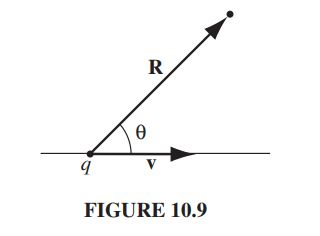
\includegraphics[height=8cm, width=8cm]{1.JPG}
      \end{center}

          \textcolor{hwColor}{
            \\
          }

    \end{enumerate}

  \pagebreak

  \item \textbf{Problem 3 [10 points]} 
  
  A transverse electric (TE) mode of frequency $\omega$ propagates along the $\hat{z}$
  direction through a hallow waveguide with square cross section of size $a$. The $z$ component of the $B$ field is
  $$
    \tilde{B}_z=B_0 ~ cos \bigg( \pi x/a \bigg) ~ cos \bigg( 2 \pi y/a \bigg) ~ exp\bigg( i k_z z-i \omega t\bigg)
  $$

    \begin{center}
      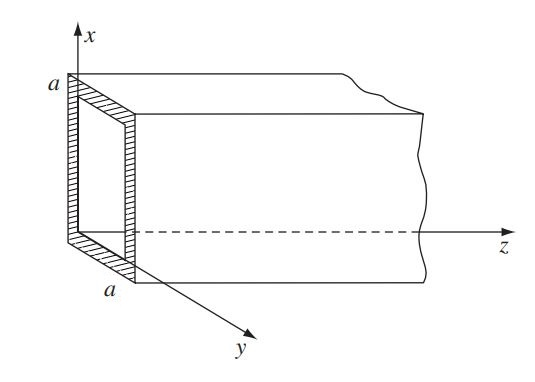
\includegraphics[height=5cm, width=5cm]{3.JPG}
    \end{center}

    \begin{enumerate}
      \item For the given mode, determine the minimum and maximum angular frequencies $\omega$ that can
      propagate through this waveguide.

        \textcolor{hwColor}{
          \\
          From the textbook, we know that if $E_z=0$, we call these TE ("transverse electric") waves. For a square wave guide shape
          which is subject to $B^{\perp}=0$ boundary condition we have:
          \\
          $
            B_z(x,y)=X(x) ~ Y(y) 
            \\
            \\
            Y \dfrac{d^2 X}{dx^2}+X \dfrac{d^2 Y}{dy^2}+\left[\bigg( \omega/c \bigg)^2-k^2\right] XY=0
            \Longrightarrow \begin{cases}
              \dfrac{1}{X} \dfrac{d^2 X}{dx^2}=-k^2_x
              \\
              \\
              \dfrac{1}{Y} \dfrac{d^2 Y}{dy^2}=-k^2_y
            \end{cases}
            \\
            \\
            \\
            \text{The General solution: } X(x)=A ~ sin\bigg( k_x x\bigg)+b ~ cos \bigg( k_x x\bigg)
            \\
            \\
            \text{Based on the boundry condition A is zero therefore}, 
            \\
            \\
            \therefore ~~~ \begin{cases}
              B_z=B_0 ~ cos\bigg( m \pi x/a\bigg) ~ cos\bigg( n \pi y/a\bigg), ~~~~ m,n=0,1,2,...
              \\
              \\
              k=\sqrt{
                \bigg( \omega/c \bigg)^2- \pi^2 \left[ \bigg( m/a \bigg)^2+\bigg( n/b \bigg)^2 \right]
              }
            \end{cases}
            \\
            \\
            \\
            \\
            \\
          $
          From the textbook, this result is called $T_{mn}$ mode. Comparing the above result with the given 
          transverse electric mode gives us $m=1$ and $n=2$.
          \\
          \\
          $
            k=\sqrt{\bigg( \omega/c \bigg)^2- \pi^2 \left[ \bigg( 1/a \bigg)^2+\bigg( 2/a \bigg)^2 \right]}
            =\sqrt{\bigg( \omega/c \bigg)^2- \pi^2 \left[ 1/a^2 + 4/a^2 \right]}
            \\
            \\
            \\
            \therefore ~~~ \boxed{
              k=\sqrt{\bigg( \omega/c \bigg)^2- \dfrac{5 \pi^2}{a^2}}
            } ~~~ \checkmark
          $
          \\
          \\
          \\
          $
            \text{The cutoff frequency is } \omega < c \pi \sqrt{\bigg( m/a \bigg)^2+\bigg( n/a \bigg)^2} \equiv \omega_{mn}
            \\
            \\
            \\
            \omega_{mn}=c \pi \sqrt{\dfrac{m^2+n^2}{a^2}}=c \pi \dfrac{\sqrt{m^2+n^2}}{\sqrt{a^2}}
            \Longrightarrow \omega_{mn}=\dfrac{c \pi}{a} \sqrt{m^2+n^2}
            \\
            \\
            \\
            \omega_{12}=\dfrac{c \pi}{a} \sqrt{1^2+2^2}
            \\
            \\
            \\
            \therefore ~~~ \boxed{
              \omega_{12}=\dfrac{c \pi}{a} \sqrt{5}
            } ~~~~ \checkmark ~~~~
          $
          This is the lowest cutoff frequency.
          \\
          \\
          \\
          \textbf{Sanity check:}
          \\
          $
            \text{If } \omega=\dfrac{c \pi}{a} \sqrt{5} \text{ then } k=\sqrt{\bigg( \bigg( \dfrac{c \pi}{a} \sqrt{5} \bigg) /c \bigg)^2- \dfrac{5 \pi^2}{a^2}}=0
            \\
            \\
          $
          If $\omega$ is less than that then the wave number is imaginary. I do not think there is a maximum angular frequency since any
          larger values for $\omega$ keeps the wave number a real number.
          \\
          \\
        }

      \item Determine the time-averaged flux of field energy passing through the waveguide. \emph{Hint: It will
      save you some time to note that, as I pointed out in lecture, the time-averaged Poynting vector
      could be simplified to read} $\langle S \rangle=\dfrac{1}{2 \mu_0} ~ Re \bigg( E_0 \times B^*_0 \bigg)$

        \textcolor{hwColor}{
          \\
          \\
          $
            \langle S \rangle=\dfrac{1}{2 \mu_0} ~ Re \bigg( E_0 \times B^*_0 \bigg)
            \\
            \\
            \\
            \tilde{B}_z=B_0 ~ cos \bigg( \pi x/a \bigg) ~ cos \bigg( 2 \pi y/a \bigg) ~ e^{i( k_z z-\omega t)}
            \\
            \\
            \therefore ~~~ \boxed{
              B_z=B_0 ~ cos \bigg( \pi x/a \bigg) ~ cos \bigg( 2 \pi y/a \bigg) cos(k_z z-\omega t)
            } ~~~~ \checkmark
            \\
            \\
            \\
            \text{Since this is a TE mode } \boxed{E_z=0}. 
            \\
            \\
            E.q ~ (9.180)
            \\
            \\
            \begin{cases}
              E_x=\dfrac{i}{(\omega/c)^2 -k^2} \bigg( k \dfrac{\partial E_z}{\partial x}+\omega \dfrac{\partial B_z}{\partial y} \bigg)
              =\dfrac{i}{(\omega/c)^2 -k^2} \bigg( k \dfrac{\partial ~ 0}{\partial x}+\omega \dfrac{\partial}{\partial y} \left[B_0 ~ cos \bigg( \pi x/a \bigg) ~ cos \bigg( 2 \pi y/a \bigg)\right] \bigg)
              \\
              \\
              E_y=\dfrac{i}{(\omega/c)^2 -k^2} \bigg( k \dfrac{\partial E_z}{\partial y}-\omega \dfrac{\partial B_z}{\partial x} \bigg)
              =\dfrac{i}{(\omega/c)^2 -k^2} \bigg( k \dfrac{\partial ~ 0}{\partial y}-\omega \dfrac{\partial}{\partial x} \left[B_0 ~ cos \bigg( \pi x/a \bigg) ~ cos \bigg( 2 \pi y/a \bigg)\right]  \bigg)
              \\
              \\
              B_x=\dfrac{i}{(\omega/c)^2 -k^2} \bigg( k \dfrac{\partial B_z}{\partial x}-\dfrac{\omega}{c^2} \dfrac{\partial E_z}{\partial y} \bigg)
              =\dfrac{i}{(\omega/c)^2 -k^2} \bigg( k \dfrac{\partial}{\partial x} \left[B_0 ~ cos \bigg( \pi x/a \bigg) ~ cos \bigg( 2 \pi y/a \bigg)\right]  -\dfrac{\omega}{c^2} \dfrac{\partial ~ 0}{\partial y} \bigg)
              \\
              \\
              B_y=\dfrac{i}{(\omega/c)^2 -k^2} \bigg( k \dfrac{\partial B_z}{\partial y}+\dfrac{\omega}{c^2} \dfrac{\partial E_z}{\partial x} \bigg)
              =\dfrac{i}{(\omega/c)^2 -k^2} \bigg( k \dfrac{\partial}{\partial y} \left[B_0 ~ cos \bigg( \pi x/a \bigg) ~ cos \bigg( 2 \pi y/a \bigg)\right] +\dfrac{\omega}{c^2} \dfrac{\partial ~ 0}{\partial x} \bigg)
            \end{cases}
            \\
            \\
            \\
            \begin{cases}
              E_x=-\dfrac{i}{(\omega/c)^2 -k^2} \bigg( \dfrac{2 \pi \omega B_0}{a} cos(\dfrac{\pi x}{a}) ~ sin(\dfrac{2 \pi y}{a}) \bigg)
              \\
              \\
              E_y=\dfrac{i}{(\omega/c)^2 -k^2} \bigg( \dfrac{\pi \omega B_0}{a} sin(\dfrac{\pi x}{a}) ~ cos(\dfrac{2 \pi y}{a}) \bigg)
              \\
              \\
              B_x=-\dfrac{i}{(\omega/c)^2 -k^2} \bigg( \dfrac{\pi k B_0}{a} sin(\dfrac{\pi x}{a}) ~ cos(\dfrac{2 \pi y}{a}) \bigg) 
              \\
              \\
              B_y=-\dfrac{i}{(\omega/c)^2 -k^2} \bigg( \dfrac{2 \pi k B_0}{a} cos(\dfrac{\pi x}{a}) ~ sin(\dfrac{2 \pi y}{a}) \bigg)
            \end{cases}
            \\
            \\
            \\
            \\
            \therefore ~~~ \begin{cases}
              E_x=-\dfrac{i}{(\omega/c)^2 -k^2} \bigg( \dfrac{2 \pi \omega B_0}{a} cos(\dfrac{\pi x}{a}) ~ sin(\dfrac{2 \pi y}{a}) \bigg)
              \\
              \\
              E_y=\dfrac{i}{(\omega/c)^2 -k^2} \bigg( \dfrac{\pi \omega B_0}{a} sin(\dfrac{\pi x}{a}) ~ cos(\dfrac{2 \pi y}{a}) \bigg)
              \\
              \\
              E_z=0
              \\
              \\
              B^*_x=\dfrac{i}{(\omega/c)^2 -k^2} \bigg( \dfrac{\pi k B_0}{a} sin(\dfrac{\pi x}{a}) ~ cos(\dfrac{2 \pi y}{a}) \bigg) 
              \\
              \\
              B^*_y=\dfrac{i}{(\omega/c)^2 -k^2} \bigg( \dfrac{2 \pi k B_0}{a} cos(\dfrac{\pi x}{a}) ~ sin(\dfrac{2 \pi y}{a}) \bigg)
              \\
              \\
              B^*_z=B_0 ~ cos \bigg( \pi x/a \bigg) ~ cos \bigg( 2 \pi y/a \bigg)
            \end{cases}
            \\
            \\
            \Longrightarrow \langle S \rangle=\dfrac{1}{2 \mu_0} ~ \bigg( E_0 \times B^*_0 \bigg)
            =\dfrac{1}{2 \mu_0} ~ \left[
              \hat{x} \bigg( E_y B^*_z - E_z B^*_y \bigg)
              -\hat{y} \bigg( E_x B^*_z - E_z B^*_x \bigg)
              +\hat{z} \bigg( E_x B^*_y - E_y B^*_x \bigg)
            \right]
            \\
            \\
            \\
            =\dfrac{1}{2 \mu_0} ~ \left[
              \hat{x} \bigg( E_y B^*_z \bigg)
              -\hat{y} \bigg( E_x B^*_z \bigg)
              +\hat{z} \bigg( E_x B^*_y - E_y B^*_x \bigg)
            \right]
            \\
            \\
            \\
            =\dfrac{1}{2 \mu_0} \times \bigg(
              \hat{x} \bigg( \dfrac{i}{(\omega/c)^2 -k^2} \dfrac{\pi \omega B^2_0}{a} sin(\dfrac{\pi x}{a}) ~ cos(\dfrac{\pi x}{a}) ~ cos^2(\dfrac{2 \pi y}{a}) \bigg)
              \\
              \\
              \\
              -\hat{y} \bigg( -\dfrac{i}{(\omega/c-k^2)^2 }  \dfrac{2 \pi \omega B^2_0}{a} sin(\dfrac{2 \pi y}{a}) cos(\dfrac{2 \pi y}{a}) cos^2(\dfrac{\pi x}{a}) \bigg)
              \\
              \\
              \\
              +\hat{z} \bigg(
                \dfrac{4 \pi^2 \omega B^2_0 k}{\left[(\omega/c)^2-k^2\right]^2 a^2} cos^2(\dfrac{\pi x}{a}) sin^2(\dfrac{2 \pi y}{a})
                 -
                 \dfrac{- \pi^2 \omega k B^2_0}{\left[(\omega/c)^2-k^2\right]^2 a^2} sin^2(\dfrac{\pi x}{a}) cos^2(\dfrac{2 \pi y}{a})
              \bigg)
            \bigg)
            \\
            \\
            \\
            \\
            \bigints\limits_{0}^{a} \bigints\limits_{0}^{a} ~ \langle S \rangle dx ~ dy
            \\
            \\
            \text{Using } \bigints\limits_{0}^{a} sin^2(m \pi/a) dx=\bigints\limits_{0}^{a} cos^2(m \pi x/a) dx=\dfrac{a}{2} \text{ we have:}
            \\
            \\
            \\
            \Longrightarrow   \bigints\limits_{0}^{a} \bigints\limits_{0}^{a} ~ \langle S \rangle dx ~ dy
            =\dfrac{1}{8 \mu_0} \dfrac{\pi^2 k \omega B^2_0}{\left[(\omega/c)^2-k^2\right]^2} \left[ 
              \bigg( \dfrac{1}{a} \bigg)^2+\bigg( \dfrac{2}{a} \bigg)^2
            \right]
            \\
            \\
            \\
            \\
            \therefore ~~~ \boxed{
              \bigints\limits_{0}^{a} \bigints\limits_{0}^{a} ~ \langle S \rangle dx ~ dy
              =\dfrac{5}{8 \mu_0} \dfrac{\pi^2 k \omega B^2_0}{\left[(\omega/c)^2-k^2\right]^2 ~ a^2}
            } ~~~~ \checkmark
            \\
          $
        }

    \end{enumerate}

  \pagebreak

  \item \textbf{Problem 4 [10 points]} 
  
  A transverse electric (TE) mode of frequency $\omega$ propagates along the $\hat{z}$ direction through a hollow
  waveguide with square cross section of size $a$. The $z$ component of the $B$ field is
  $$
    \tilde{B}_z=B_0 ~ cos \bigg( \pi x/a \bigg) ~ cos \bigg( \pi y/a \bigg) ~ exp\bigg( i k z-i \omega t\bigg)
  $$
  We take the real part of the above to be the actual field strength.
    \begin{enumerate}
      \item Write down the dispersion relation $k(\omega)$ and determine the group and phase velocities.

        \textcolor{hwColor}{
          \\
          $
            \tilde{B}_z=B_0 ~ cos \bigg( \pi x/a \bigg) ~ cos \bigg( \pi y/a \bigg) ~ e^{i(kz-\omega t)}
            \\
            \\
            \text{The real part} ~~~ \boxed{
              B_z=B_0 ~ cos \bigg( \pi x/a \bigg) ~ cos \bigg(\pi y/a \bigg) cos(k z-\omega t)
            } ~~~~ \checkmark
            \\
            \\
          $
          Basically, a dispersion relation is a representation of a wave's frequency as a function of wavelenght which
          is more common to use angular frequency $\omega$ and the wave number instead of frequency and wavelenght.
          $B_z=B_0 ~ cos(\dfrac{m \pi x}{a}) ~ cos(\dfrac{n \pi y}{b})$ is called the solution of $TE_{mn}$ mode.
          From the lecture notes we know (for a TE wave)
          \\
          \\
          $
            \begin{cases}
              \omega_{mn}=c \pi \sqrt{\bigg( \dfrac{m}{a} \bigg)^2+\bigg( \dfrac{n}{b} \bigg)^2}
              \\
              \\
              k(\omega)=\dfrac{1}{c} \sqrt{\omega^2-\omega^2_{mn}}
              \\
              \\
              v_{phase}=\dfrac{\omega}{k}=\dfrac{c}{\sqrt{1-\bigg( \omega_{mn}/\omega \bigg)^2}}
              \\
              \\
              v_{group}=\dfrac{1}{dk/d\omega}
            \end{cases}
            \Longrightarrow
            \dfrac{dk}{d \omega}=\dfrac{d}{d \omega} \left[
              \dfrac{1}{c} \sqrt{\omega^2-\omega^2_{mn}}
            \right]=\dfrac{\omega}{c \sqrt{\omega^2-\omega^2_{mn}}}
            \\
            \\
            \\
            \begin{cases}
              \omega_{mn}=\dfrac{c \pi}{a} \sqrt{2}
              \\
              \\
              k(\omega)=\dfrac{1}{c} \sqrt{\omega^2-\dfrac{2 c^2 \pi^2}{a^2}}
              \\
              \\
              v_{phase}=\dfrac{c}{\sqrt{1-\dfrac{2 c^2 \pi^2}{a^2 \omega^2}}}
              \\
              \\
              v_{group}=\dfrac{1}{dk/d\omega}=\dfrac{1}{\dfrac{\omega}{c \sqrt{\omega^2-\omega^2_{mn}}}}
              =\dfrac{c \sqrt{\omega^2-\omega^2_{mn}}}{\omega}
            \end{cases}
            \\
            \\
          $
          I am a bit doubtful about my results because I am not sure if I used the correct formula for $B_z$ in both 
          questions 3 $\&$ 4. The reason is that the textbook has defined $B_0 ~ cos(m \pi x/a) ~ cos(n \pi y/b)$ so the 
          values for $m$ and $n$ are clear. In the two questions, I used $e^{i(kz-\omega t)}$ otherwise, I'd end up
          with $B_0 ~ cos \bigg( \pi x/a \bigg) ~ cos \bigg(\pi y/a \bigg) cos(k z-\omega t)$ which I was not sure how to 
          retrieve the values of $m$ and $n$. The only way that I could think of was to use 
          \emph{Angle-Sum and -Difference Trig Identities} to make $cos \bigg( \pi x/a \bigg) ~ cos \bigg(\pi y/a \bigg) cos(k z-\omega t)$
          similiar to $cos(m \pi x/a) ~ cos(n \pi y/b)$ from the textbook and then continue the work. I hope my solutions are worth
          some points. Thank you!
          \\
          \\
        }

      \item Determine the surface charge density $\rho(y,z,t)$ for the wall of the waveguide with surface normal
      in the $\hat{n}=-\hat{x}$ direction. Hint: you should firstly write down a general expression for the
      surface charge density on the surface of an ideal conductor. Assume the waveguide is an ideal
      conductor.

        \textcolor{hwColor}{
          \\
        }
  
    \end{enumerate}

  \pagebreak

  \item \textbf{Problem 5 [20 points]}
  
  A straight, neutral wire of length $L$ carries a line current of $I ~ \hat{x}$ along the $\hat{x}$ axis for times
  $t \ge 0$  (it is suddenly turned on). The current is zero everywhere for times $t < 0$. As a result of the current,
  point charges accumulate at the ends of the wire, at the positions $r=0$ and $r=-L ~ \hat{x}$. The point charges
  are initially zero, for times $t < 0$. Determine the vector potential $A(t)$, the scalar potential $V(t)$, the
  electric field $E(t)$ and the magnetic field $B(t)$ at the position $r=x_0 \hat{x}$. Assume $L >> x_0 > 0$, and 
  write your solutions only for the time domain $t < L/c$ (in other words, you may pretend that the
  wire is infinitely long).
  \begin{center}
    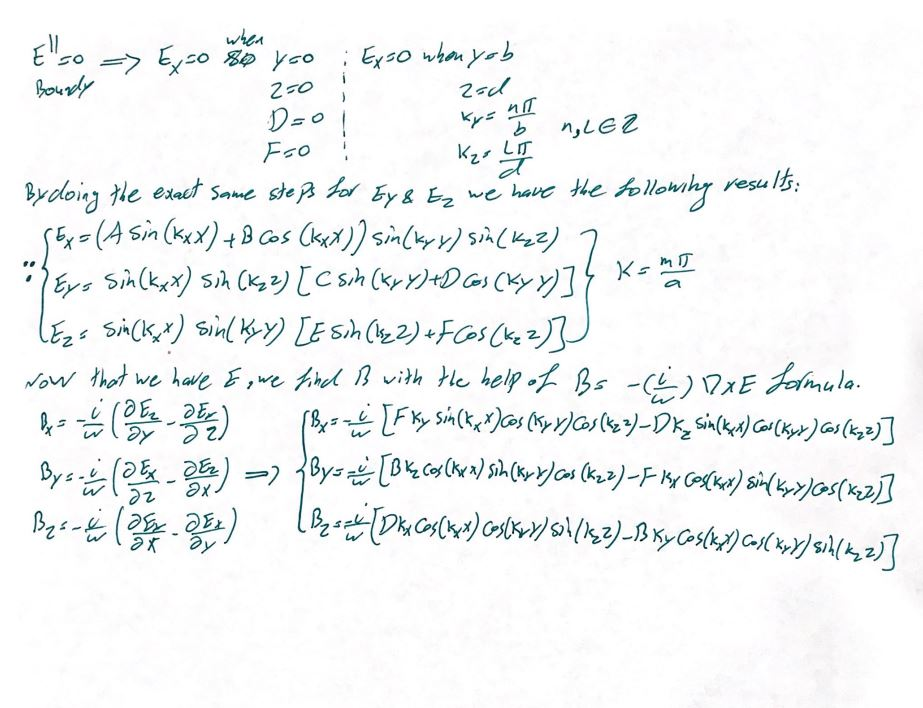
\includegraphics[height=3cm, width=12cm]{2.JPG}
  \end{center}

      \textcolor{hwColor}{
        \\
        $
          I=\begin{cases}
            I ~ \hat{x} ~~~~ t \geq 0
            \\
            \\
            0 ~~~~~~ t <0
          \end{cases}
          \\
          \\
          \\
        $
        Since the wire is electircally neutral, so the scalr potential $V$ is zero everywhere ourtside the wire. 
        We leanred that in the nonstatic case, it is not the status of the source \emph{right now} that matters,
        but rather its condition at some earlier at the retarded, $t_r$, time when the message left. $\scriptr$ 
        is always the distance from the source point to the field point, so we have:
        \\
        \\
        $
          t_r=t-\dfrac{\scriptr}{c}
          \\
          \\
          \\
          A=\hat{x} ~ \dfrac{\mu_0}{4 \pi} \bigints\limits_{X_1}^{X_2} ~ \dfrac{J \bigg( r^', t-\dfrac{\scriptr}{c} \bigg)}{\scriptr} ~ dx
          =\hat{x} ~ \dfrac{\mu_0}{4 \pi} \bigints\limits_{X_1}^{X_2} ~ \dfrac{I(t_r)}{\scriptr} ~ dx
          \\
          \\
        $
        For the field to reach point $P$ which is $x_0$ away from the end of the wire, takes $\dfrac{x_0}{c}$ so for $t < \dfrac{x_0}{c}$
        $A=0$. 
        \\
        \\
        $
          A=2\bigg( \hat{x} ~ \dfrac{\mu_0 I}{4 \pi} \bigg) \bigints\limits_{x_0}^{ct-s} \dfrac{1}{ x-L } ~ dx
          \\
          \\
          \\
          \therefore ~~~ \boxed{
            A=\dfrac{\mu_0 I}{2 \pi} ln \bigg( \dfrac{ct-s-L}{x_0-L} \bigg) ~ \hat{x}
          } ~~~~ \checkmark
        $
        \\
        \\
        \\
        Knowing $A$, we can calculate $E$ and $B$.
        \\
        \\
        $
          \begin{cases}
            B=\nabla \times A=\dfrac{\partial A_x}{\partial s} ~ \hat{\phi}=\dfrac{\partial}{\partial s} \left[\dfrac{\mu_0 I}{2 \pi} ln \bigg( \dfrac{ct-s-L}{x_0-L} \bigg) \right] ~ \hat{\phi}
            \\
            \\
            E=-\dfrac{\partial A}{\partial t}
            =-\dfrac{\partial}{\partial t} \left[\dfrac{\mu_0 I}{2 \pi} ln \bigg( \dfrac{ct-s-L}{x_0-L} \bigg)\right] ~ \hat{x}
          \end{cases}
          \\
          \\
          \\
          \\
          \therefore ~~~ \boxed{
            B=\dfrac{\mu_0 I}{2 \pi \bigg( ct-s-L \bigg)} ~ \hat{\phi}
            ~~~~~~~
            E=-\dfrac{\mu_0 I c}{2\pi \bigg( ct-s-L \bigg)} ~ \hat{x}
          } ~~~~ \checkmark
          \\
          \\
        $
      }

  \item \textbf{Problem 6 [20 points]}

  A laser of frequency $\omega$ shines at normal incidence on a thin metal film with properties $\epsilon, \mu, \sigma$. 
  The complex wavenumber within the conductor is $\tilde{k}= a + ib$. Assume a vacuum outside of the film.
    \begin{enumerate}
      \item Assuming the high-conductivity limit, determine what a and b are. Don't derive anything; use
      the formula sheet.

        \textcolor{hwColor}{
          \\
          From the textbook on page 412, for a \emph{prefect} conductor we have $\rho=\infty$ and $\tau=0$.
          \\
          \\
          $
            \begin{cases}
              \tilde{k}=a+ib
              \\
              \\
              a \equiv \omega \sqrt{\dfrac{\epsilon \mu}{2}} \left[ \sqrt{1+\bigg( \dfrac{\sigma}{\epsilon \omega} \bigg)^2+1} \right]^{1/2}
              \\
              \\
              b \equiv \omega \sqrt{\dfrac{\epsilon \mu}{2}} \left[ \sqrt{1+\bigg( \dfrac{\sigma}{\epsilon \omega} \bigg)^2-1} \right]^{1/2}
            \end{cases}
          $
          \\
          \\
          \\
          From chapters 4, 6, and 7 we learned the following:
          \\
          \\
          $
            \begin{cases}
              \epsilon=\epsilon_r \epsilon_0
              \\
              \\
              \mu=\mu_0 \bigg( 1+ \chi_m \bigg)
            \end{cases}
            \\
            \\
            \\
            \therefore ~~~ \boxed{
              \tilde{k}=\omega \left[
                \sqrt{\dfrac{\epsilon \mu}{2}} \left[ \sqrt{1+\bigg( \dfrac{\sigma}{\epsilon \omega} \bigg)^2+1} \right]^{1/2}
              +i ~ \sqrt{\dfrac{\epsilon \mu}{2}} \left[ \sqrt{1+\bigg( \dfrac{\sigma}{\epsilon \omega} \bigg)^2-1} \right]^{1/2}
              \right]
            }
          $
        }

      \item Determine the electric field $E(z,t)$ and magnetic field $B(z,t)$ within the conductor, assuming
      the incident beam has an electric field $E_I= \hat{x} ~ E_{I0} ~ exp \bigg( i k_0 z - i \omega t \bigg)$ 
      and the metal-vacuum interface is at $z = 0$. You don't need to derive anything; use the formula sheet. 
      You may write your answer in terms of the symbols $a$ and $b$.

      \textcolor{hwColor}{
        \\
        $
          \begin{cases}
            \tilde{E}(z,t)=\tilde{E}_{I0} ~ e^{\tilde{k}z-\omega t}
            =\tilde{E}_{I0} ~ e^{-bz} ~ e^{i(kz-\omega t)} ~ \hat{x}
            \\
            \\
            \tilde{B}(z,t)=\tilde{B}_0 ~ e^{\tilde{k}z-\omega t}
            =\dfrac{a+ib}{\omega} ~ \tilde{E}_{I0} ~ e^{-bz} ~ e^{i(az-\omega t)} ~ \hat{y}
          \end{cases}
          \\
          \\
        $
        \\
        The \emph{real} B and E are:
        \\
        \\
        $
          \begin{cases}
            E(z,t)=\tilde{E}_{I0} ~ e^{-bz} ~ cos(az-\omega t+\delta_E) ~ \hat{x}
            \\
            \\
            B(z,t)=\tilde{E}_{I0} ~ e^{-bz} ~ cos(kz-\omega t+\delta_E+\phi) ~ \hat{y}
          \end{cases}
          \\
          \\
          \\
        $
        where 
        $
          \\
          \\
          \dfrac{B_0}{E_0}=\dfrac{\sqrt{a^2+b^2}}{\omega}=\sqrt{\epsilon \mu \sqrt{1+(\dfrac{\sigma}{\epsilon \omega})^2}}
          \\
          \\
          \\
          \phi=Arctan\big( \dfrac{b}{a} \bigg)
          \\
          \\
          \\
          \delta-B-\delta_E=\phi
          \\
          \\
        $
      }

    \end{enumerate}

  \end{enumerate}

\end{document}
